\documentclass[ngerman,hyperref={pdfpagelabels=false}]{beamer}

% -----------------------------------------------------------------------------

\graphicspath{{images/}}

% -----------------------------------------------------------------------------

\usetheme{KIT}

\setbeamercovered{transparent}
%\setbeamertemplate{enumerate items}[ball]

\newenvironment<>{KITtestblock}[2][]
{\begin{KITcolblock}<#1>{#2}{KITblack15}{KITblack50}}
{\end{KITcolblock}}

\usepackage[ngerman,english]{babel}
\usepackage[utf8]{inputenc}
\usepackage[TS1,T1]{fontenc}
\usepackage{array}
\usepackage{multicol}
\usepackage[absolute,overlay]{textpos}
\usepackage{beamerKITdefs}
\usepackage[ruled,vlined,linesnumbered,norelsize]{algorithm2e}

\pdfpageattr {/Group << /S /Transparency /I true /CS /DeviceRGB>>}	%required to prevent color shifting withd transparent images


\title{SAT Solving with distributed local search}
\subtitle{Guangping Li -- \textit{uzdif@student.kit.edu}}

\author[Guangping Li]{Guangping Li}
\institute{Institute of Theoretical informatics, Algorithmics II}

\TitleImage[width=\titleimagewd,height=\titleimageht]{titel}

\KITinstitute{Institute of Theoretical informatics}
\KITfaculty{KIT Department of Informatics}

% -----------------------------------------------------------------------------

\begin{document}
\setlength\textheight{7cm} %required for correct vertical alignment, if [t] is not used as documentclass parameter


% title frame
\begin{frame}
  \maketitle
\end{frame}


% intro
\section{Presentation}
\begin{frame}
  \frametitle{Outline}

\heading{ \color<beamer:2>{red}{propositional satisfiability problem (\emph{\textbf{SAT}})}}
  \begin{itemize}
  \item Notations
  \item Local Search in SAT Problem
  \end{itemize}
\heading{Solving SAT by swpSolver}
  \begin{itemize}
  \item Basic scheme
  \item Data structure
  \item Our improvements
  \end{itemize}
\heading{Our Parallel SAT-solver}
  \begin{itemize}
  \item The pure portfolio approach
  \item Two failures
  \item Initialization with a guide of formula partitioning
  \end{itemize}
\heading{Conclusion}
  
\end{frame}


% blocks
\begin{frame}
	\frametitle{The vertex coloring problem}

	\begin{KITalertblock}{vertex coloring}
	\begin{itemize}
	\item  The goal is to color the vertices of an undirected graph such that no two adjacent vertices share the same color. 
	\end{itemize}
	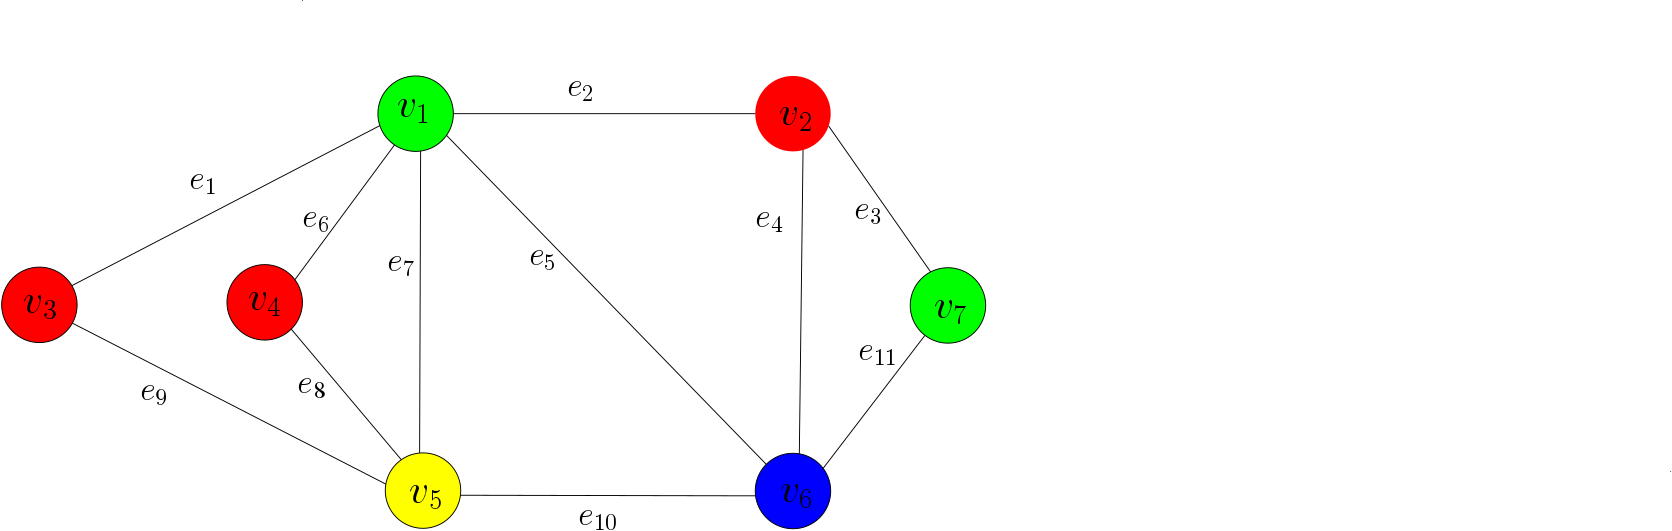
\includegraphics[scale=0.2]{1/nodeColoring1}
	\end{KITalertblock}

\end{frame}
\begin{frame}
	\frametitle{The vertex coloring problem}

	\begin{KITinfoblock}{k-vertex coloring problem}
	\begin{itemize}
		\item A $k$-vertex coloring of a graph is a function $c$: $V\rightarrow \{1...k\}$. 
	\end{itemize}
	\begin{figure}
	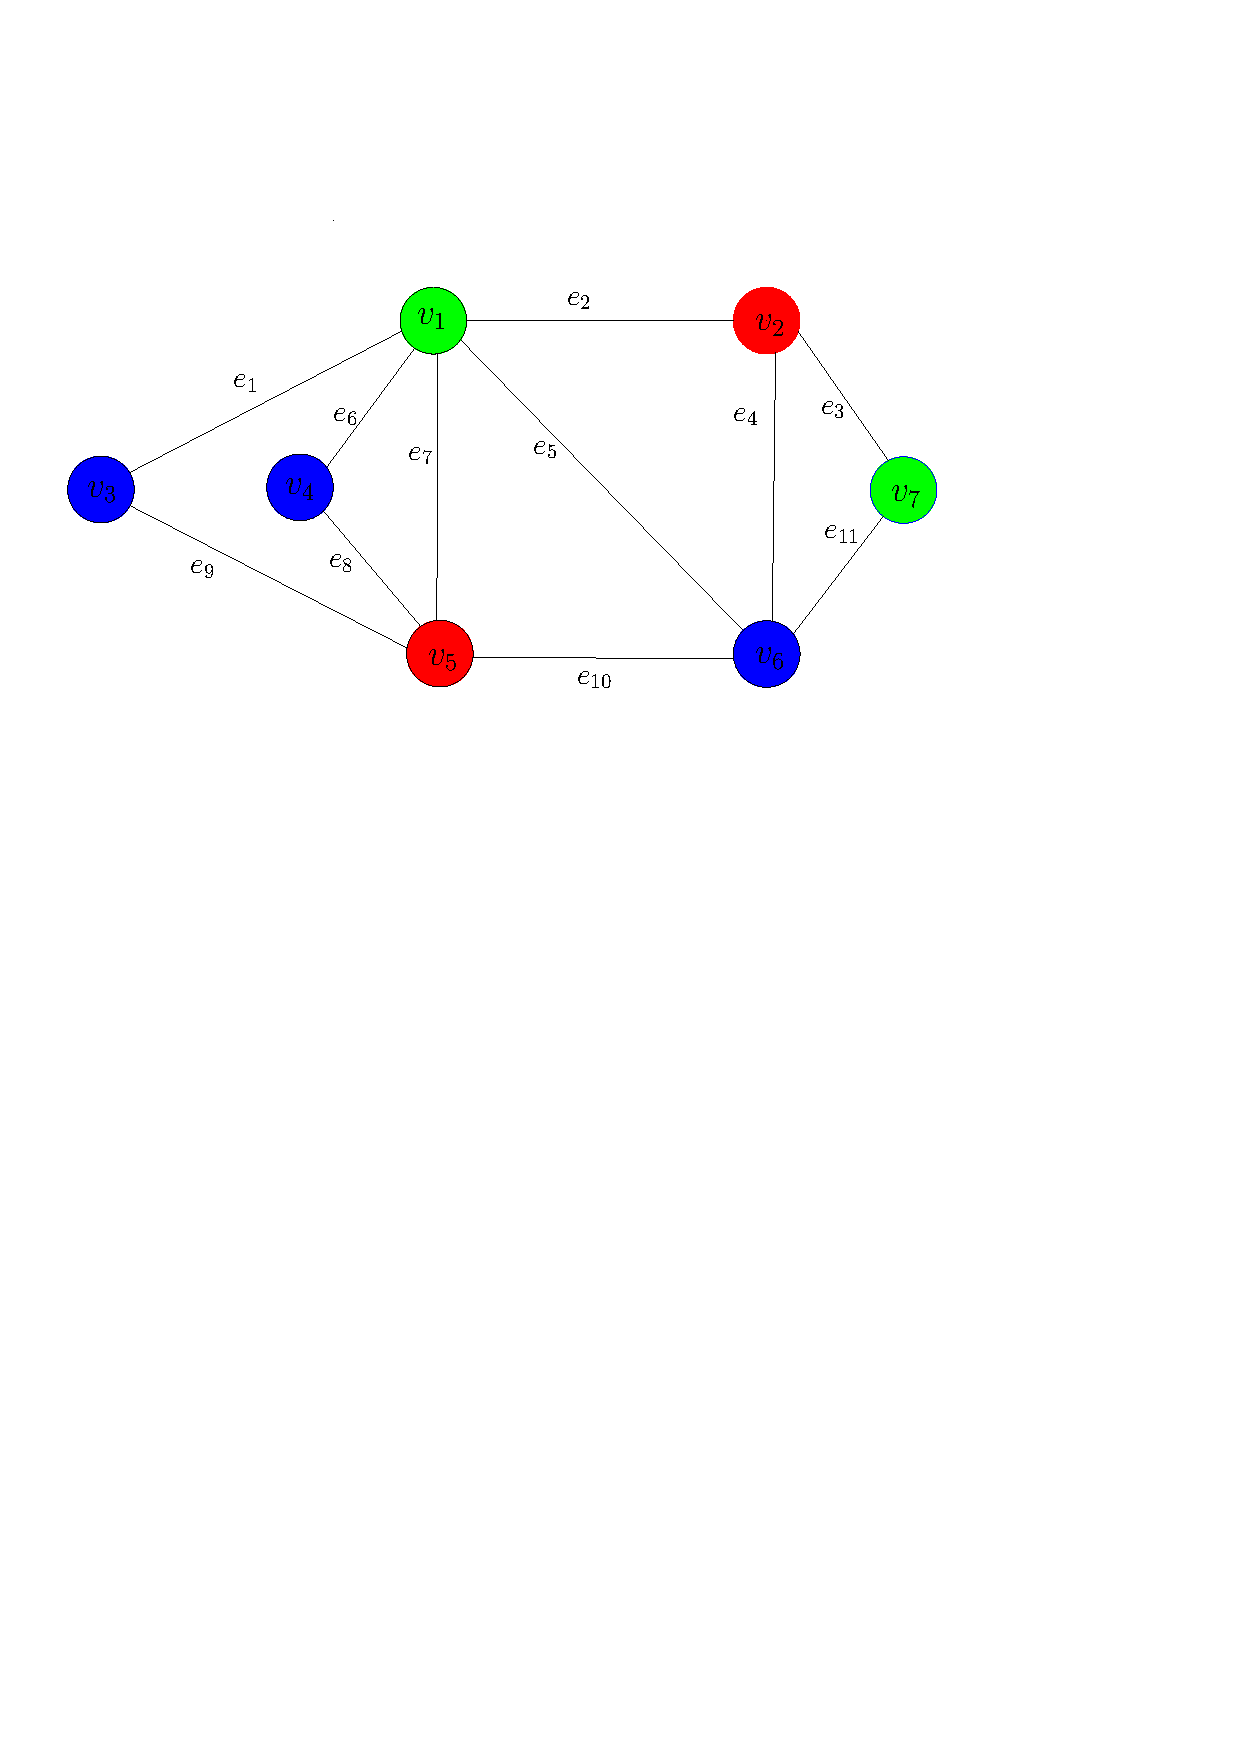
\includegraphics[scale=0.2]{1/nodeColoring2}
	\caption{a legal 4-coloring}
	\end{figure}	
	\end{KITinfoblock}
\end{frame}
\begin{frame}
	\frametitle{The vertex coloring problem}
	
	\begin{KITexampleblock}{Vertex coloring problem}
	\begin{itemize}
		\item The \emph{\textbf{VCP}} is to determine the smallest $k$, such that the graph can be colored using $k$ colors without conflicts. 
		\item This lower bound $k$ is called the \emph{\textbf{chromatic number}} of G, denoted by $\chi(G)$.
	\end{itemize}
	\end{KITexampleblock}
\end{frame}
\begin{frame}
  \frametitle{Outline}

\heading{The vertex coloring problem}
  \begin{itemize}
  \item k-VCP
  \item VCP
  \end{itemize}
  
\heading{\color<beamer:1>{red}{The Tabucol algorithm}}
\heading{Solving VCP by Tabucol}
  \begin{itemize}
  \item Basic scheme
  \item Data structure
  \item Our improvements
  \end{itemize}
\heading{Our Parallel GCP-solver}
  \begin{itemize}
  \item Parameter combinations
  \item Our approaches
  \end{itemize}
\heading{Conclusion}
\end{frame}


% blocks continued
\begin{frame}
	\frametitle{The Tabucol algorithm}
	\framesubtitle{solving k-VCP}
	  \begin{itemize}
  \item Introduced in 1987 by Hertz and de Werra 
  \item The local search will start from an initial $k$-coloring $c$.
  \item Changing the color of one vertex to color, is called \emph{\textbf{one-step move}}.
  \item the best move with most reduction of conflicts will be reached.
  \item To avoid short-term cycling, recently performed moves are marked as forbidden moves for a given duration.
  \end{itemize}
\end{frame}
	
\begin{frame}
	\frametitle{The Tabucol algorithm}	
The pseudo code of \emph{\textbf{Tabucol}}:

\begin{algorithm}[H]
\SetKwInOut{Input}{input}
\SetKwInOut{Output}{output}
\SetKwInOut{Parameter}{parameter}
 \Input{A Graph $G=\{V,E\}$, an integer $k>0$}
 \Parameter{$L$, $\alpha$, $Timeout$}
 \Output{Coloring $c$}
 Build a random $k$-coloring $c'$:\\
 $c$ = $c'$;\\
 $i = 0$;\\
 \While {$(f(c)\neq 0$ $ \land$ Timeout does not occur$)$}{
  Evaluate all permitted one-step-moves of $c$ with function $\Gamma$;\\
  Choose the move [v,i] with maximum $\Gamma(c, v,i)$; \\
  Mark the corresponding one-step move [v,i] as a forbidden move with duration $L+\alpha \times f(c)$;\\
  Change $c(v) = i$; \
 }
 \caption{Algorithm Tabucol}
\end{algorithm}

\end{frame}
\begin{frame}
  \frametitle{Outline}

\heading{The vertex coloring problem}
  \begin{itemize}
  \item k-VCP
  \item VCP
  \end{itemize}
  
\heading{{The Tabucol algorithm}}
\heading{\color<beamer:1>{red}{Solving VCP by Tabucol}}
  \begin{itemize}
  \item Basic scheme
  \item Data structure
  \item Our improvements
  \end{itemize}
\heading{Our Parallel VCP-solver}
  \begin{itemize}
  \item Parameter combinations
  \item Our approaches
  \end{itemize}
\heading{Conclusion}
\end{frame}


% drawing area
\begin{frame}
	\frametitle{Solving VCP by Tabucol}
	\framesubtitle{Basic scheme}
	  \begin{columns}[T]
    \begin{column}{.4\textwidth}
     \begin{block}{}
    \begin{itemize}
    \item Step 1: Initialize Coloring
    \item Step 2: Solve k-VCP
    \item Step 3: Reduce a color
    \end{itemize}
    \end{block}
    \end{column}
    \begin{column}{.6\textwidth}
    \begin{block}{}
% Your image included here
    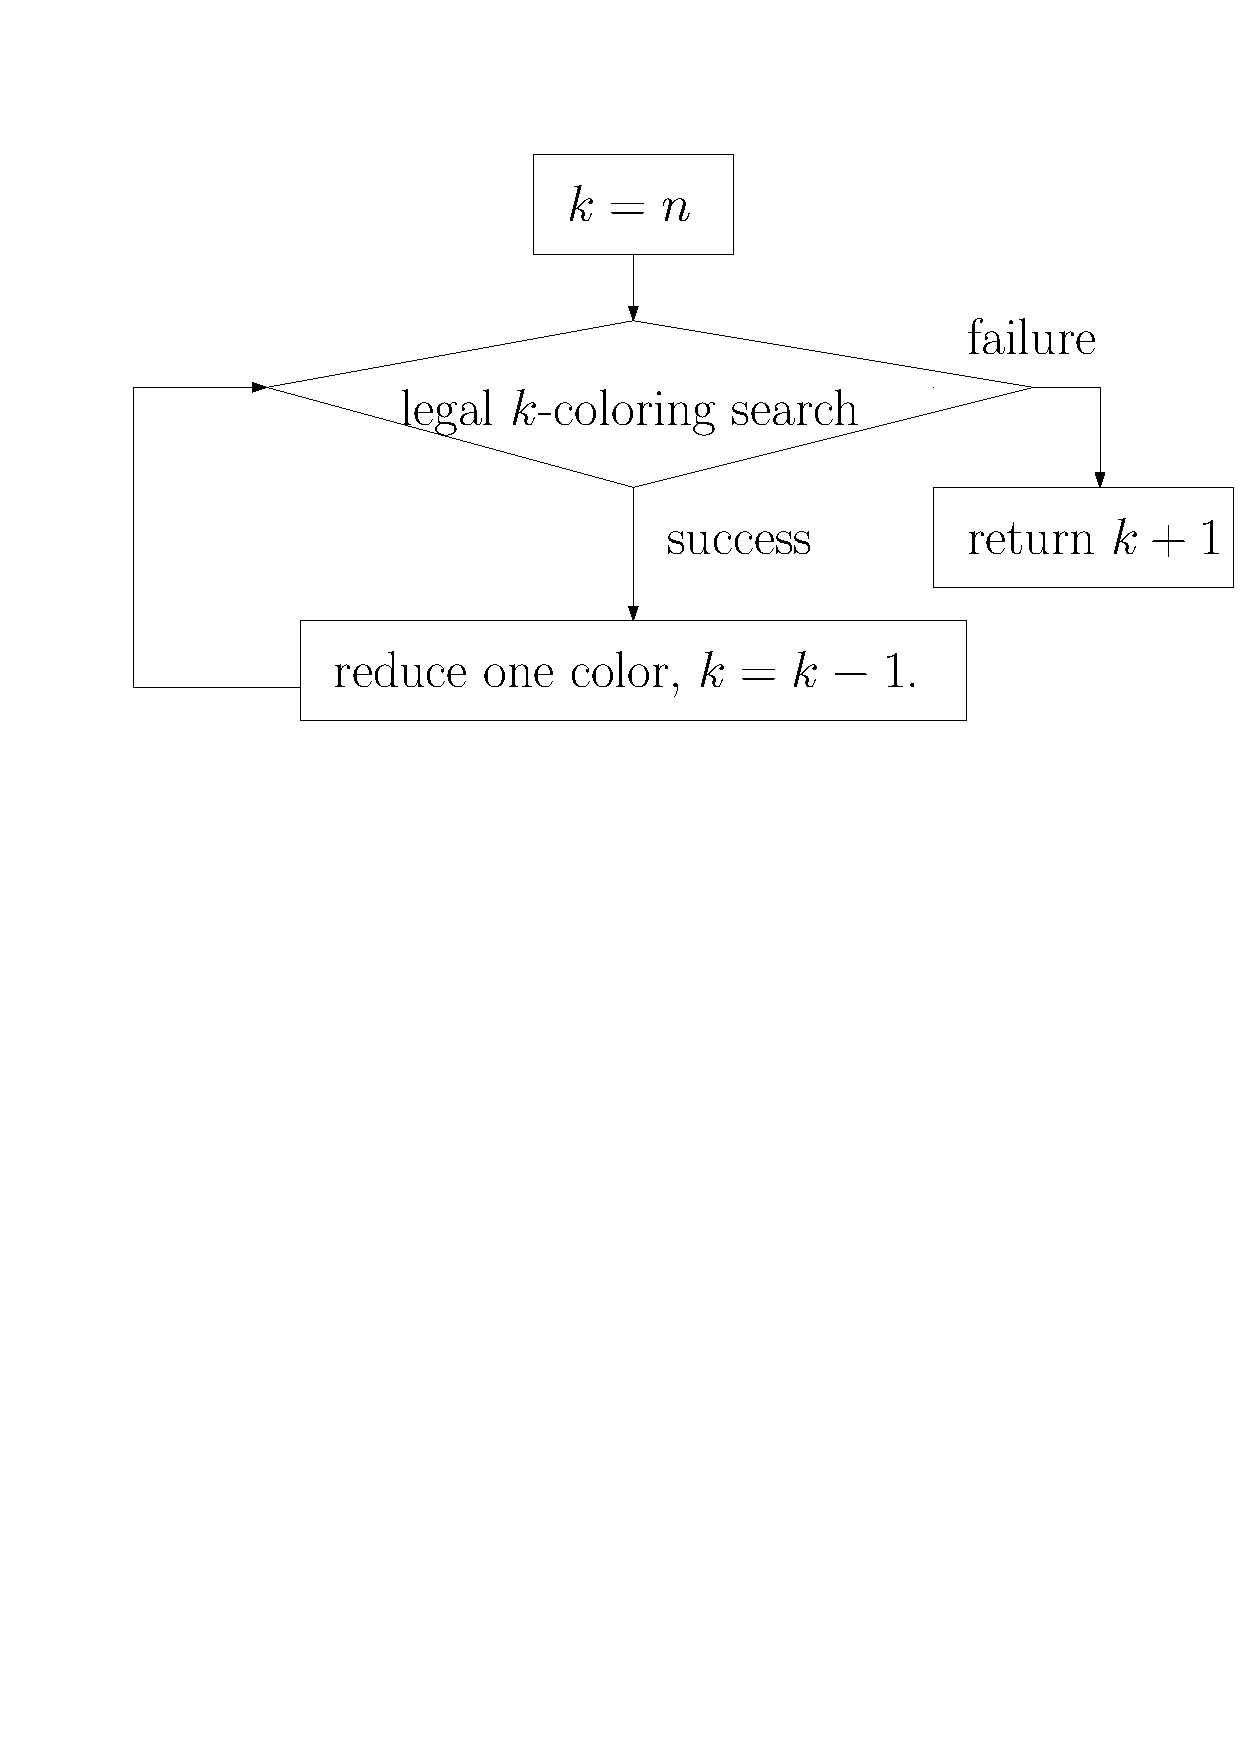
\includegraphics[scale=0.35]{1/gcpSolver.pdf}
    \end{block}
    \end{column}
  \end{columns}
\end{frame}

\begin{frame}
	\frametitle{Data structure}
	\begin{KITalertblock}{ Tabu Map and Tabu Queue }
	\begin{itemize}

	\item To avoid using the forbidden candidates, a hash map should provide whether a candidate is a tabu or not.
	\item  A one-step move [v, i] is represented by an ordered pair $(v, i) $.\\
\item to update the forbidden moves stored in the \emph{Tabu Map}.
\item The size of the \emph{Tabu Queue} is $L+ f(n)\times \alpha$.
\item When the color of a vertex $v$ is changed, $(v,c(v))$ is recorded in the  \emph{Tabu Map} and also enqueued in the \emph{Tabu Queue}.
\item When the \emph{Tabu Queue} is full, extra forbidden moves  will be popped and will be deleted in the \emph{Tabu Map}.\\
	\end{itemize}
	\end{KITalertblock}
\end{frame}

\begin{frame}
	\frametitle{Data structure}
	\begin{KITalertblock}{ Solution matrix}
	\begin{itemize}
\item To reuse the calculated results, a matrix $M$ is used to record the information about the neighborhood.  \item The matrix $M$  evaluates the candidate moves of the current $k$-coloring $c$.
\item If $c(v_j) = i$, $M_{ij}$ is the number of conflicting edges incident to $v_j$ in the current solution.
\item $\frac{\sum_{j=1}^n M_{c(v_j)j}}{2}$ is the conflict number of solution $c$;
\item If $c(v_j)\neq i$, $M_{ij}$ is the number of conflicts involving $v_j$ in a neighbor coloring $c'$ of $c$ with\\
$c'(v_j) = i$.\\
 $c'(v_q) = c(v_q), q \neq i,q \in \{1..n\}.$ \\
	\end{itemize}
	\end{KITalertblock}
\end{frame}
\begin{frame}
	\frametitle{Data structure}
	\begin{KITalertblock}{ Solution matrix}
	\begin{itemize}
\item $\Gamma(j,i)=M_{c(v_{j})j}-M_{ij}$ evaluates the improvement of the move $[j, i]$ in constant time.
\item This matrix is filled at the beginning based on the initial solution and constantly changed. 
\item If the chosen one-step move is $[i, j]$, which means changing the color of $v_i$ from current color $c(v_i)$ to $j$, some entities in matrix $M$ must be updated. 

	\end{itemize}
	\end{KITalertblock}
\end{frame}

\begin{frame}
\frametitle{Evaluation}
\begin{itemize}
\item {The 68 graphs used in our experiments are from the DIMACS benchmark collection.}
\item {The single-threaded experiments were run on computers that had four AMD(R) Opteron(R) processors 6168 (1.9 Ghz with 12 cores) and 256GB RAM. The computers ran the 64-bit version of Ubuntu 12.04.}
\item{ The multi-threaded experiments were run on fat nodes InstitutsClusterII. IC2 is a distributed memory parallel computer with 480 16-way so-called thin compute nodes and 5 32-way so-called fat compute nodes. The thin nodes are equipped with 16 cores, 64 GB main memory, whereas the fat nodes are equipped with 32 cores, 512 GB main memory.}
	\end{itemize}
\end{frame}

\begin{frame}
\frametitle{Evaluation}
\begin{itemize}
\item {An advantage plot shows the advantage of an algorithms to another algorithm. The y-axis gives the ordered percentage differences.}
	\end{itemize}
	\begin{figure}
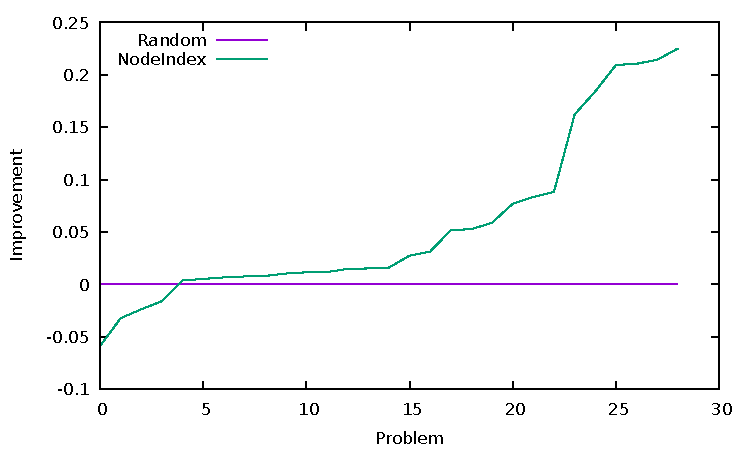
\includegraphics[scale=0.4]{Experiments/E1/imp/impro.pdf}
\end{figure}
\end{frame}

\begin{frame}
	\frametitle{Our improvements}
	\heading{Basic scheme}
    \begin{itemize}
    \item Step 1: Initialize Coloring (How to initialize coloring?)
    \item Step 2: Solve k-VCP (How to improve Tabucol?)
    \item Step 3: Reduce a color (How to reconstruct coloring?)
    \end{itemize}
\end{frame}
\begin{frame}
	\frametitle{Solving VCP by Tabucol}
    \framesubtitle{Step 1:How to initialize coloring?}
    	\begin{KITexampleblock}{     Our Node-index initialization vs Random initialization }
\begin{itemize}
\item
\textbf{Node-index initialization} is to use c: $v_i \rightarrow i$ as the initial solution. 
\item
\textbf{Random initialization} is to build a coloring randomly.
\end{itemize} 
\begin{figure}
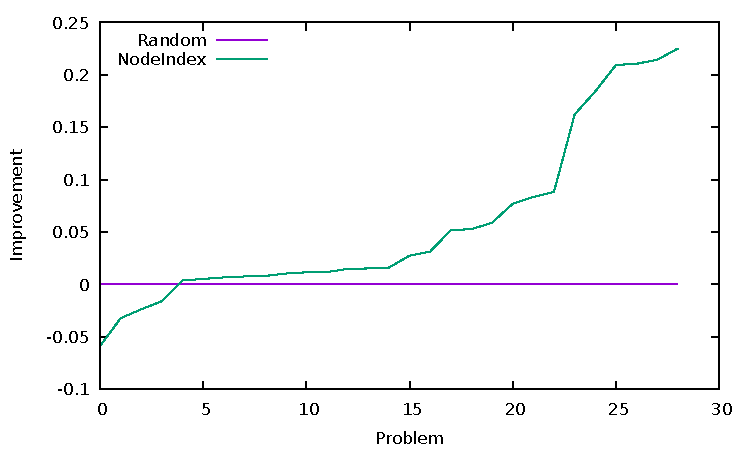
\includegraphics[scale=0.4]{Experiments/E1/imp/impro.pdf}
\end{figure}
\end{KITexampleblock}
\end{frame}
\begin{frame}
	\frametitle{Solving VCP by Tabucol}
    \framesubtitle{Step 2: How to improve Tabucol?}
    \begin{KITexampleblock}{ Our column-traverse vs row-traverse of solution matrix}
    \begin{itemize}
\item
To find next move, the maximum element in the solution matrix must be found. 
\item If more than one candidate exists, the first found one is chosen as the next step.
\item This matrix can be traversed row by row or column by column.  
    \end{itemize} 
 \begin{figure}
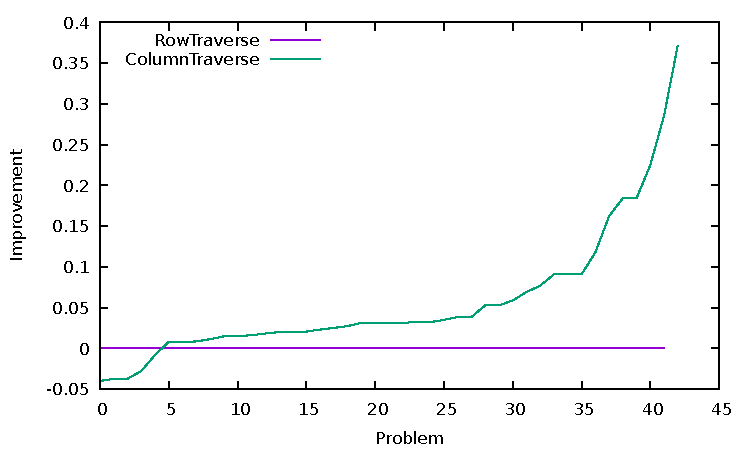
\includegraphics[scale=0.4]{Experiments/E3/imp/impro.pdf}
\end{figure}   
\end{KITexampleblock}
\end{frame}
\begin{frame}
	\frametitle{Solving VCP by Tabucol}
    \framesubtitle{Step 2: How to improve Tabucol?}
    \begin{KITexampleblock}{ Statistic matrix}
    \begin{itemize}
\item The Tabucol algorithm uses a tabu list to avoid short-term cycling.
\item To recognize long-term cycling, a \emph{statistic matrix S} is added. 
\item The $S_{ij}$ represents how many times a one-step move $[i,j]$ was chosen as the next step. 
\item The candidate with the smallest statistic value will be chosen in the next step.  
    \end{itemize} 
 \begin{figure}
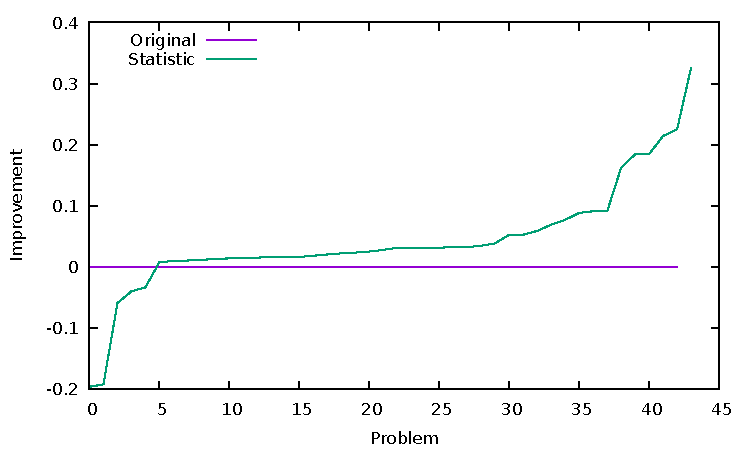
\includegraphics[scale=0.4]{Experiments/E4/imp/impro.pdf}
\end{figure}   
\end{KITexampleblock}
\end{frame}
\begin{frame}
	\frametitle{Solving VCP by Tabucol}
    \framesubtitle{Step 3: How to reconstruct new coloring?}
\begin{KITexampleblock}{An observation}
It seems that the solution loses its potential in the process of reducing colors iteratively. So it should be helpful to use a new and perhaps more potential coloring.
\end{KITexampleblock}
 \begin{KITexampleblock}{Replace by a randomly generated solution}
We replace the current illegal solution  occasionally by a new randomly generated coloring of the same size.
 \begin{figure}
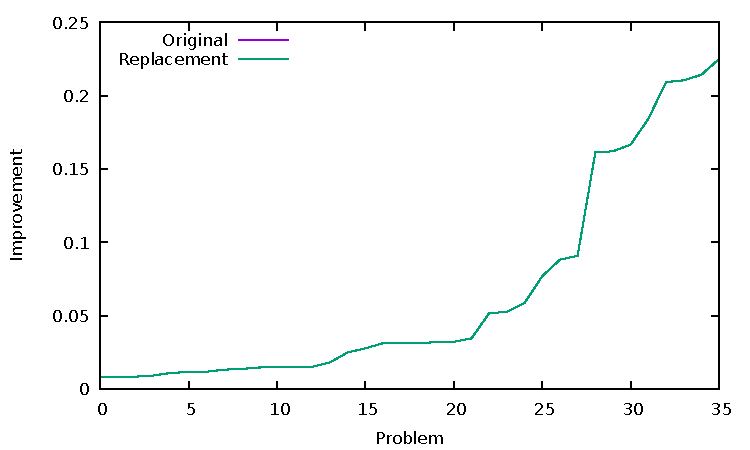
\includegraphics[scale=0.4]{Experiments/E2/imp/impro.pdf}
\end{figure}   
\end{KITexampleblock}
\end{frame}
\begin{frame}
  \frametitle{Outline}

\heading{The vertex coloring problem}
  \begin{itemize}
  \item k-VCP
  \item VCP
  \end{itemize}
\heading{{The Tabucol algorithm}}
\heading{Solving VCP by Tabucol}
  \begin{itemize}
  \item Basic scheme
  \item Data structure
  \item Our improvements
  \end{itemize}
\heading{\color<beamer:1>{red}{Our Parallel GCP-solver}}
  \begin{itemize}
  \item Parameter combinations
  \item Our approaches
  \end{itemize}
        \heading{Conclusion}
\end{frame}
\begin{frame}
	\frametitle{Our Parallel GCP-solver}
    \framesubtitle{Parameter combinations}
    \begin{itemize}
    \item Most graphs get better results with the our suggestions. 
\item Some graphs get better results with the original GCP-solver.
    \item The agents run with different combinations of the suggestions ($L$, $\alpha$, the search directions and whether a statistic matrix is introduced).
    \end{itemize}
\end{frame}
\begin{frame}
	\frametitle{Our Parallel GCP-solver}
    \framesubtitle{Parameter combinations}
    \small
      \begin{tabular}{| l | l l l l l l |p{2cm}|}
   \hline
Index&L& $\alpha$ &Initialization&Replace&Traverse& Statistic\\ \hline
1&9 &0.38 &Node-Index&true&Column&true\\
2&1 &0.77&Node-Index&true&Column&true\\
3&11 &0.90&Node-Index&true&Column&true \\
4&17 &0.59&Random&true&Column&true \\
5&18 &0.42&Node-Index&false&Column&false\\\hline
6&4 &0.92&Node-Index&true&Column&true \\
7&16 &0.76&Node-Index&false&Row&false\\
8&17 &0.47&Node-Index&false&Column&false\\
9&2 &0.60&Node-Index&true&Column&false\\
10&2 &0.54&Node-Index&false&Column&true\\\hline
11&5 &0.46&Random&true&Column&true\\
12&11 &0.63&Random&true &Column&true\\
13&7 &0.83&Node-Index&true&Column&true\\
14&8 &0.98&Node-Index&false &Row&true\\
15&18 &0.58&Node-Index&true&Column&false \\
16&13 &0.90&Node-Index&false&Column&true \\\hline
    \end{tabular}
\end{frame}
\begin{frame}
	\frametitle{Our Parallel GCP-solver}
    \framesubtitle{Parameter combinations}
    \small
      \begin{tabular}{| l | l l l l l l |p{2cm}|}
   \hline
Index&L& $\alpha$ &Initialization&Replace&Traverse& Statistic\\ \hline

17&20 &0.56&Node-Index&true &Column&false\\
18&10&0.95&Node-Index&true &Column&true\\
19&15 &0.55&Node-Index&true&Row&true\\
20&17 &0.39&Node-Index&true&Column&true \\\hline
21&18 &0.52&Node-Index&false&Column&true\\
22&11 &0.32&Node-Index&true&Column&true \\
23&15 &0.62&Node-Index&false&Column&true \\
24&6 &0.94&Random&true&Column&true\\
25&9 &0.94&Node-Index&false&Column &false\\\hline
26&12 &0.96&Node-Index&true&Column&true\\
27&16 &0.58&Node-Index&false&Column&true\\
28&9 &0.45&Node-Index&false&Column&true\\
29&19 &0.95&Node-Index&true&Column&true \\
30&18 &0.31&Node-Index&true&Column &false\\\hline
31&6 &0.50&Node-Index&false&Column&false\\
32&15 &0.93&Node-Index&false&Column &false\\\hline
    \end{tabular}
\end{frame}
\begin{frame}
	\frametitle{Our Parallel GCP-solver}
    \framesubtitle{1st Approach: The pure portfolio approach}
    \begin{itemize}
\item The agents run the GCP solver with different parameter combinations. 
\item After collecting the solutions found by each agent, the search takes the coloring of the minimum size as the result.
    \end{itemize}
\end{frame}
\begin{frame}
	\frametitle{Our Parallel GCP-solver}
    \framesubtitle{2nd Approach: Forced color reducing}
\begin{itemize}
\item This approach is based on the pure portfolio approach.
\item The agents share the minimum size.
\item One agent has already found a $k$-coloring and broadcasts it.
\item With this notification, all agents search for a legal $k-1$ coloring.
\end{itemize}
\begin{figure}
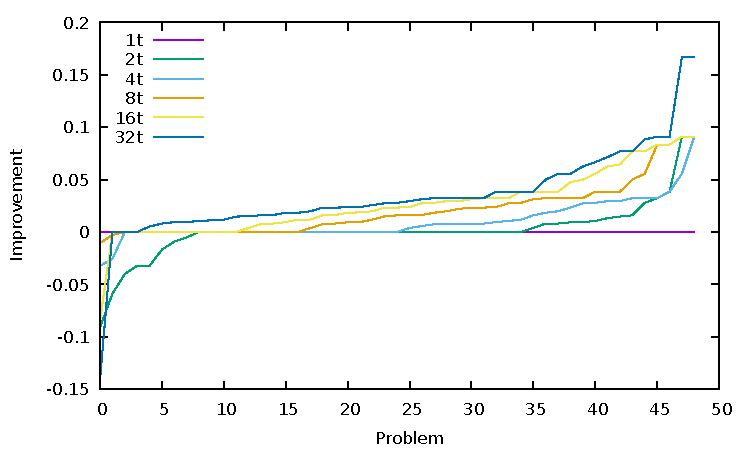
\includegraphics[scale=0.6]{Experiments/E6/imp/impro.pdf}
\end{figure}
\end{frame}

\begin{frame}
	\frametitle{Our Parallel GCP-solver}
    \framesubtitle{3rd Approach: Tabu sharing}
    \begin{itemize}
\item A tabu list records the search path to avoid short-term cycling.
\item The agents share the ``traps'' of local search loops. 
    \end{itemize}
 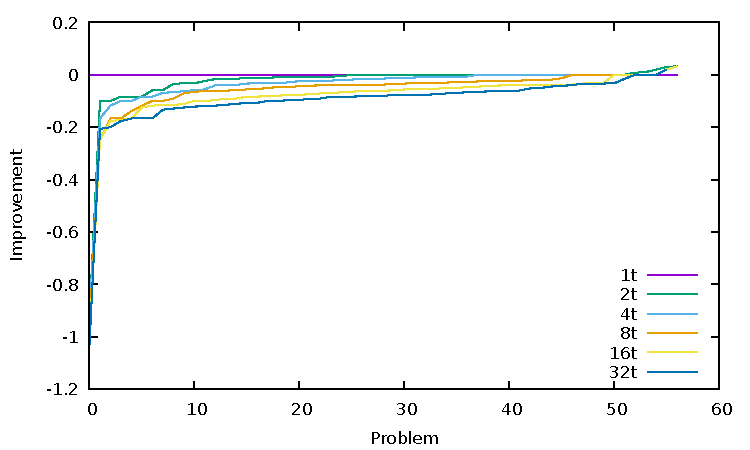
\includegraphics[scale=0.6]{Experiments/E7/imp/impro.pdf}
\end{frame}

\begin{frame}
	\frametitle{Our Parallel GCP-solver}
    \framesubtitle{4th Approach: Statistic sharing}
\begin{itemize}
\item To recognize long-term cycling, a \emph{statistic matrix S} is added. 
\item The $S_{ij}$ represents how many times a one-step move $[v_i,j]$ was chosen as the next step. 
\item The candidate with the smallest statistic value will be chosen in the next step.  
\item The agents use one common statistic matrix.\\
  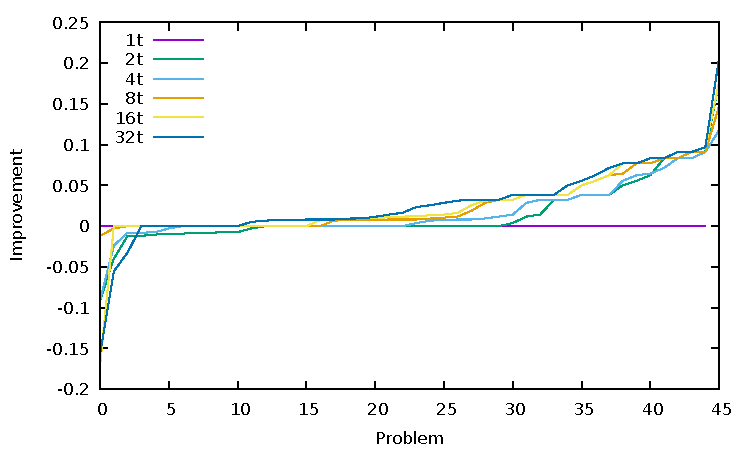
\includegraphics[scale = 0.6]{Experiments/E8/imp/impro.pdf}
\end{itemize}
\end{frame}
\begin{frame}
  \frametitle{Outline}

\heading{The vertex coloring problem}
  \begin{itemize}
  \item k-VCP
  \item VCP
  \end{itemize}
  
\heading{The Tabucol algorithm}
\heading{Solving VCP by Tabucol}
  \begin{itemize}
  \item Basic scheme
  \item Data structure
  \item Our improvements
  \end{itemize}
\heading{Our Parallel GCP-solver}
  \begin{itemize}
  \item Parameter combinations
  \item Our approaches
  \end{itemize}
\heading{ \color<beamer:1>{red}Conclusion} 
\end{frame}
\begin{frame}
	\frametitle{Conclusion}
\heading{Our improvement:}
\begin{itemize}
\item An algorithm solves the VCP with parallel Tabucol searches.
\item The statistic matrix recognizes long-term cycling and brings improvement to our algorithm.
\item Certain information exchange (minimum size, statistic matrix) can improve the performance of the parallel search. 
\end{itemize}

\heading{Comparison of our GCP-solver with DSATUR, PASS, TRICK:} 
\begin{itemize}
\item  50 of 68 (73\%) benchmark graphs get best results with our solver.
\item  20 of 68 (29\%) benchmark graphs get unique best results with our solver.
\end{itemize}
\heading{Further work}
\begin{itemize}
\item Using different  search strategies
\item Using different cooperation strategies
\item Using different algorithms in agents
\end{itemize}
\end{frame}
\begin{frame}

 \begin{figure}

\includegraphics[scale=0.2]{1/thank-you-for-your-attention-any-questions-78.png}
\end{figure}   
\end{frame}
\end{document}
